%!TEX root = ../my_thesis.tex
\section{Correlation between systematic uncertainties}
\label{app:corrSyst}

As reported in Table~\ref{tab:summarySyst}, the main systematic uncertainties on $S_f$ and $S_{\bar f}$ are the ones due to the constraint on $\Delta m$, the fit biases, and the background subtraction. The correlations between the systematics uncertainties on $S_f$ and $S_{\bar f}$ due to these sources are described in details in this appendix. The correlation of the total systematic resulting from these three contributions is $-0.41$. The correlation between other sources of systematics is neglected.

\subsection{Correlation of $\Delta m$ systematics}
The correlation of systematics uncertainties due to $\Delta m$ between $S_f$ and $S_{\bar f}$ is estimated by comparing the nominal fit result, and the result obtained with $\Delta m$ fixed as described in Sec.~\ref{sec:systFromConsts}. This correlation $\rho^{\Delta m}_{S_f,~S_{\bar f}}$ is simply computed from the difference in statistical covariance between the two fit results:
\begin{equation}
        \rho^{\Delta m}_{S_f,~S_{\bar f}} = \frac{\sigma^{\rm nominal}_{S_f}\sigma^{\rm nominal}_{S_{\bar f}}\rho^{\rm nominal}_{S_f,~S_{\bar f}} - \sigma^{\rm\Delta m~fixed}_{S_f}\sigma^{\rm\Delta m~fixed}_{S_{\bar f}}\rho^{\rm\Delta m~fixed}_{S_f,~S_{\bar f}}}{\sqrt{(\sigma^{\rm nominal}_{S_f})^2 - (\sigma^{\rm\Delta m~fixed}_{S_f})^2}\sqrt{(\sigma^{\rm nominal}_{S_{\bar f}})^2 - (\sigma^{\rm\Delta m~fixed}_{S_{\bar f}})^2}}.
\end{equation}
The value of $\rho^{\Delta m}_{S_f,~S_{\bar f}}$ so obtained is $-1$, meaning that $S_f$ and $S_{\bar f}$ are fully anticorrelated driven by the uncertainty on $\Delta m$. This can be understood with the following argument. The $\Bzb$ versus $\Bz$ time-dependent asymmetry for the $f=\Dm\pip$ and $\bar f=\Dp\pim$ final states can be written as
\begin{align*}
  -S_f \sin(\Delta m t) + \cos(\Delta m t) &= \cos(\Delta m t + \delta_f)\,, \\
  -S_{\bar f} \sin(\Delta m t) - \cos(\Delta mt) &= -\cos(\Delta m t - \delta_{\bar f})\,,
\end{align*}
respectively, where $C_f=-C_{\bar f}=1$ is assumed, while $\delta_f = \sin^{-1}(S_f)$ and $\delta_{\bar f}=\sin^{-1}(S_{\bar f})$.
Since $S_f$ and $S_{\bar f}$ are small, the approximations $\delta_f\sim S_f$ and $\delta_{\bar f}\sim S_{\bar f}$ can be done.
As shown in Fig.~\ref{fig:amplitudes}, the sensitivity to $S_f$ and $S_{\bar f}$ is obtained around the zero of the asymmetries, 
where the cosine terms disappear. If $t_0$ is one of the zeroes, the following condition must hold:
\begin{equation}
  \label{eq:identity_dmsyst}
  \cos(\Delta m t_0 + S_f) = \cos(\pi - \Delta m t_0 + S_{\bar f}) = 0.
\end{equation}
So, if $\Delta m$ is shifted by some systematic amount, $S_f$ and $S_{\bar f}$ have to be shifted in opposite directions (and thus be anticorrelated) in order to satisfy~\ref{eq:identity_dmsyst}.

\subsection{Correlation of systematics due to fit biases}
As described in Sec.~\ref{sec:mcbootstrap}, a bias on $S_f$ and $S_{\bar f}$ is observed from bootstrapped MC samples, and the size of this bias is assigned as systematic uncertainty. The associated correlation is estimated from the two-dimensional distribution of $(S_f^{\textrm{fit}} - S_f^{\textrm{gen}})$ versus $(S_{\bar f}^{\textrm{fit}} - S_{\bar f}^{\textrm{gen}})$ obtained on the same set of bootstrapped MC samples, as shown in Fig.~\ref{fig:fitbias_corr}. The resulting correlation is $0.4$. 
\begin{figure}[t]
        \begin{center}
                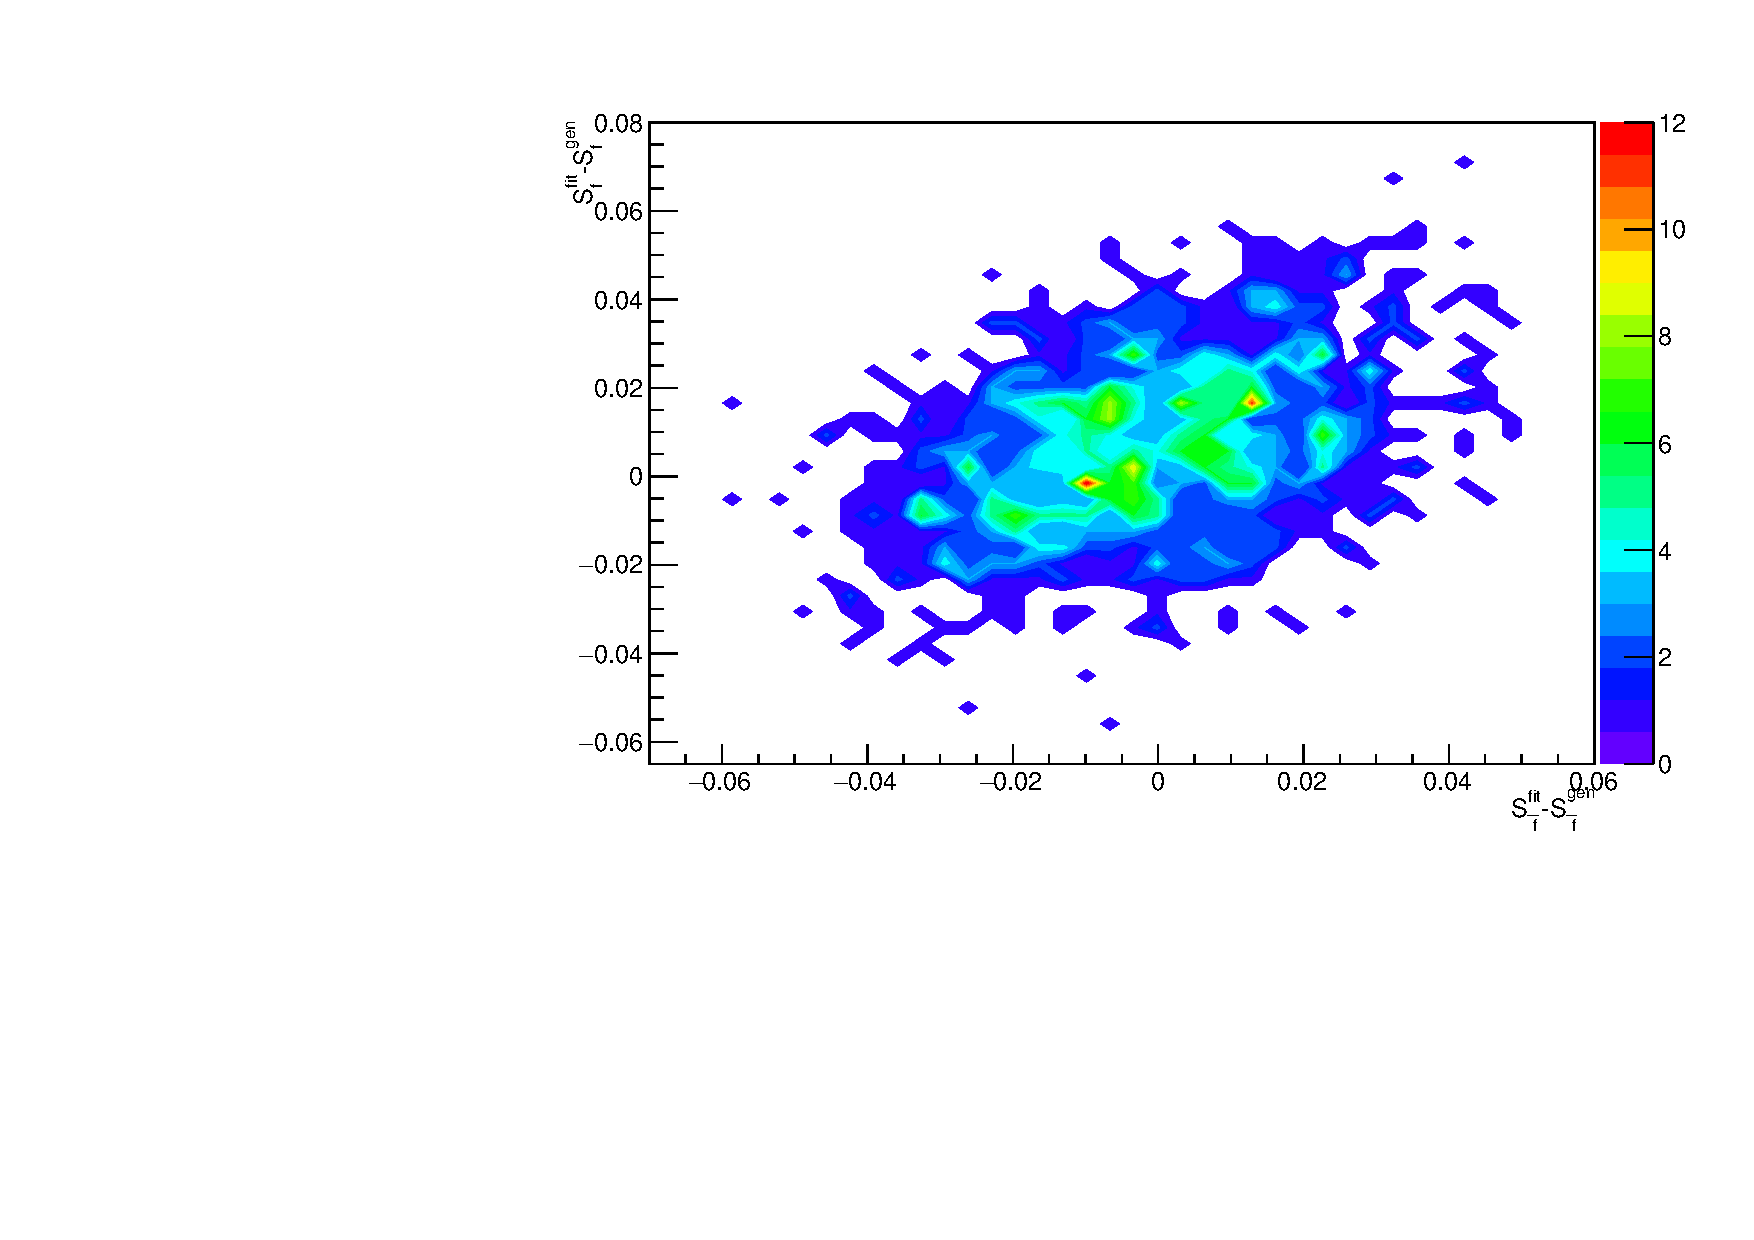
\includegraphics[width=0.7\linewidth]{AA-Appdx-corrSyst/figs/fitbias_corr.pdf}
                \end{center}
        \vspace{-2mm}
        \caption{Two-dimensional distribution of $(S_f^{\textrm{fit}} - S_f^{\textrm{gen}})$ versus $(S_{\bar f}^{\textrm{fit}} - S_{\bar f}^{\textrm{gen}})$ obtained from the fits to bootstrapped MC samples (Sec.~\ref{sec:mcbootstrap}).}
        \label{fig:fitbias_corr}
\end{figure}

\subsection{Correlation of systematics due to background subtraction}
A systematic due to \emph{sWeighting} and background subtraction is assigned by repeating Fit B in a wider mass range, as described in Sec.~\ref{sec:syst_mass}. In order to estimate the correlation of this systematic uncertainty between $S_f$ and $S_{\bar f}$, the data sample is bootstrapped in a similar way as done for the Monte Carlo (Sec.~\ref{sec:mcbootstrap}). Then, \emph{sWeights} are obtained twice on each sample, once with the nominal strategy, and once by selecting a wide mass range in Fit B. Finally, the time fit is performed on each sample using both the sets of \emph{sWeights} computed in the previous step. The correlation is estimated from the two-dimensional distribution of $(S_{\bar f}^{\textrm{nominal}} - S_{\bar f}^{\textrm{wide~mass}})$ versus $(S_f^{\textrm{nominal}} - S_f^{\textrm{wide~mass}})$, which is shown in Fig.~\ref{fig:bkgsub_corr}. The resulting correlation is $0.7$.
\begin{figure}[t]
        \begin{center}
          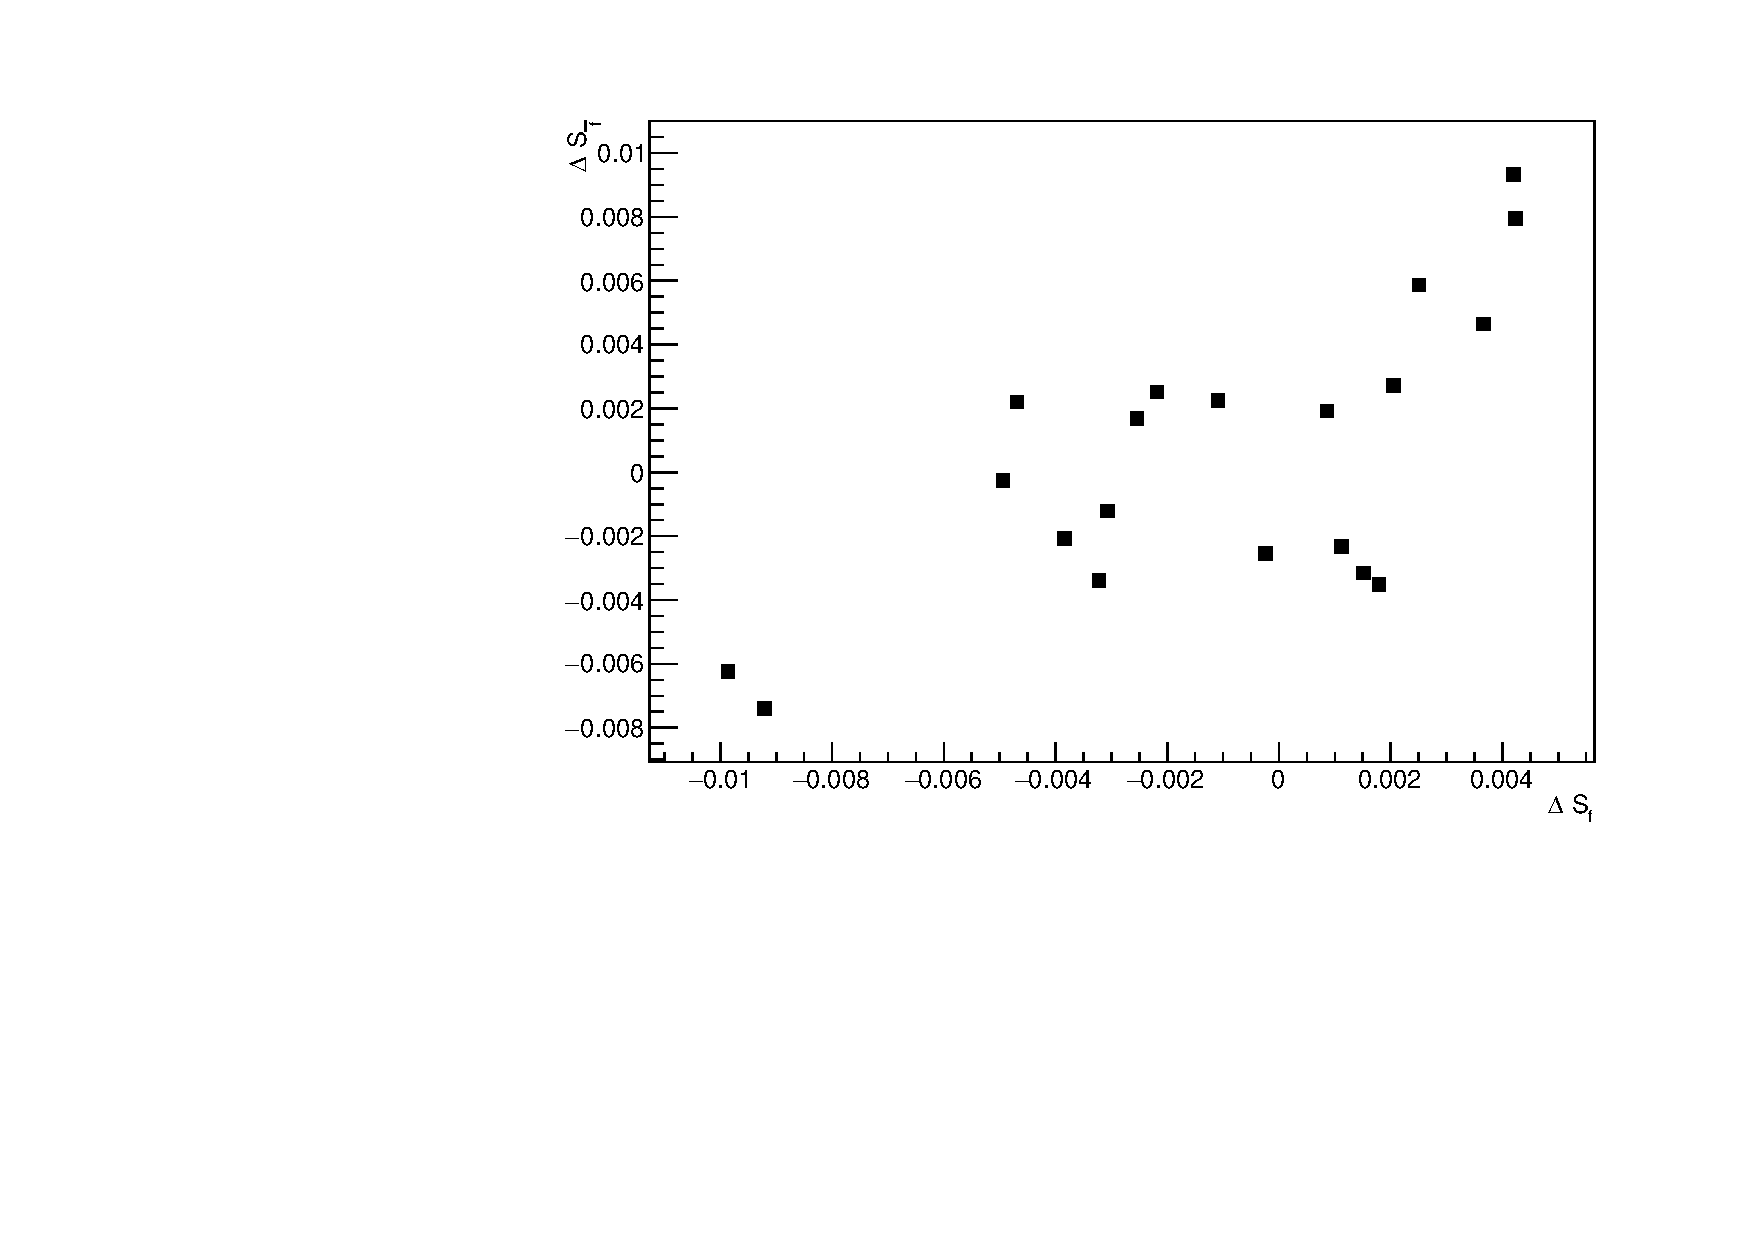
\includegraphics[width=0.7\linewidth]{AA-Appdx-corrSyst/figs/bkgsub_corr.pdf}
        \end{center}
        \vspace{-2mm}
        \caption{Two-dimensional distribution of $S_{\bar f}^{\textrm{nominal}} - S_{\bar f}^{\textrm{wide~mass}}$ ($\Delta S_{\bar f}$) versus $S_f^{\textrm{nominal}} - S_f^{\textrm{wide~mass}}$ ($\Delta S_f$) obtained from fits to bootstrapped data samples, where Fit B is performed with the nominal strategy or with a wider mass range for each sample.}
        \label{fig:bkgsub_corr}
\end{figure}
